\documentclass[11pt]{article}
\renewcommand{\rmdefault}{ptm}
\usepackage[scaled=0.92]{helvet}
\usepackage{courier,xcolor,colortbl,listings,parskip,graphicx,fancyvrb,fancyhdr,lastpage}
\usepackage{float,framed}
\normalfont
\usepackage[T1]{fontenc}
%\setlength{\parskip}{7pt}
\usepackage[toc,page]{appendix}
\usepackage[hmargin=2.5cm,vmargin=2cm]{geometry}
\usepackage[utf8]{inputenc}
\usepackage[brazil]{babel}
\usepackage{fancyvrb}
\pagestyle{fancy}
\setlength{\headheight}{120pt}
\setlength{\headsep}{30pt}
\setlength{\textheight}{550pt}
\renewcommand{\headrulewidth}{0pt}
\lhead{}
\rhead{}
\chead{
\includegraphics{brasao.jpg}\\
        \large \textbf{PRESIDÊNCIA DA REPÚBLICA}\\
        \large SECRETARIA-GERAL\\
        \large Secretaria-Executiva}
\cfoot{}
\rfoot{\thepage /\pageref{LastPage}}
\hyphenation{par-ti-ci-pa-ção}
\bibliographystyle{ieeetr}

\newcommand{\MyName}{Joenio Marques da Costa}
\newcommand{\MyEmail}{joenio@colivre.coop.br}
\newcommand{\ContractNumber}{2013/000564}
\newcommand{\ProjectCode}{Projeto PNUD BRA/12/018}
\newcommand{\NomeSecretaria}{Secretaria Geral da Presidência da República}
\newcommand{\SiglaSecretaria}{SG/PR}
\newcommand{\ProductNumber}{02}
\newcommand{\ProductDescription}{"Documento com análise de arquiteturas de
        sistemas de identidade distribuída, estratégia de implantação
        considerando os sites parceiros e contendo propostas de códigos."
}
\newcommand{\MesEntrega}{Abril de 2014}
\newcommand{\DiaEntrega}{21}

\begin{document}
\lstset{language=Ruby}
\definecolor{light-gray}{gray}{0.95}
\lstdefinestyle{codeFrame}{backgroundcolor=\color{light-gray},frame=lines}

\textbf{\ProjectCode \ -} \ProductDescription

\vspace{3cm}

\begin{minipage}{0.5\textwidth}
  \textbf{Consultora: \MyName}
  \newline
  \textbf{Contrato nº: \ContractNumber}
  \newline
  \textbf{Produto / nº: \ProductNumber}
\end{minipage}

\vspace{2cm}

\textbf{Assinatura do Consultor}

\begin{framed}
Local e data: Brasília/DF, \line(1,0){20} \ de \line(1,0){100} \ de 2014
\newline
\newline
Assinatura do Consultor: \line(1,0){300}
\end{framed}

\vspace{1cm}

\textbf{Assinatura do Supervisor}

\begin{framed}
Atesto que os serviços foram prestados conforme estabelecido no Contrato
de Consultoria.
\newline
\newline
Local e data: Brasília/DF, \line(1,0){20} \ de \line(1,0){100} \ de 2014
\newline
\newline
Assinatura e Carimbo: \line(1,0){300}
\end{framed}

\clearpage
\newcolumntype{g}{>{\columncolor{light-gray}}l}

\begin{center}
  \begin{tabular}{| g | p{10cm} |}
    \hline
    \textbf{Título} & \ProductDescription \\ \hline
    \textbf{Língua do documento} & Português - Brasil \\ \hline
    \textbf{Documentação de referência} & Português \\ \hline
    \textbf{Unidade responsável} & \NomeSecretaria \
(\SiglaSecretaria) \\ \hline
    \textbf{Criador} & \MyName - \MyEmail \\ \hline
    \textbf{Taxonomias} & Desenvolvimento \\ \hline
    \textbf{Data de aprovação} & mês de ano \\ \hline
    \textbf{Público} & \SiglaSecretaria, Parceiros e Sociedade
Civil \\ \hline
    \textbf{Aplicabilidade} & Explicar isso aqui \\ \hline
    \textbf{Faz parte do} & \ProjectCode \\ \hline
    \textbf{Em conformidade com a} & \NomeSecretaria \\ \hline
    \textbf{Documentos anexos} & Nenhum \\ \hline
    \textbf{Revisado em} & dia mês ano \\ \hline
  \end{tabular}
\end{center}

\clearpage

\tableofcontents
\clearpage
\listoffigures

\clearpage

\section{Apresentação}

Em consonância com os objetivos e cronograma previsto no âmbito do
projeto BRA/12/018:
\textbf{Desenvolvimento de Metodologias de Articulação e Gestão de
Políticas Públicas para Promoção da Democracia Participativa},
firmado entre a Secretaria-Geral da Presidência da República
(SG/PR) e o Programa das Nações Unidas para o Desenvolvimento (PNUD),
o presente documento apresenta \ProductDescription.

Essa proposta está configurada como produto \ProductNumber~da consultoria técnica
para especificação da construção dos códigos das metodologias de
organização da informação e interação participativa do portal de
participação social.


\section{SSO - Single Sign-on}

\subsection{O que é SSO?}

Single Sign-on, ou Web Browser Single Sign-on é a propriedade de controle de
acesso a sistemas de software relacionados, mas independentes. Com esta
propriedade o usuário loga apenas uma vez e ganha acesso a outros sistemas que
façam parte do mesmo ambiente de SSO sem necessidade de fornecer usuário/senha
diversas vezes. Reciprocamente, single sign-off é a propriedade do usuário
deslogar e automaticamente deslogar de outros sistemas que façam parte deste
mesmo ambiente.

Usualmente, ambientes SSO compartilham servidores de autenticação para servir
cada aplicação, com objetivo de autenticar e garantir que usuários não
necessitem entrar com usuário/senha mais de uma
vez~\footnote{http://en.wikipedia.org/wiki/Single\_sign-on}. Estes servidores
fornecem serviços de autenticação em rede para aplicações externas, a
autenticação pode ser feita por diversos métodos, mas normalmente usa-se
usuário/senha~\footnote{http://en.wikipedia.org/wiki/Authentication\_server} em
aplicações Web.

O uso de SSO aumenta drasticamente o impacto negativo em caso de roubo de
usuário/senha, uma vez que o acesso a esta informação possibilita acesso a
diversos sistemas, portanto a proteção dessas informações devem ser redobradas.
É preciso também ter cuidado com a disponibilidade deste serviço, uma vez
que sua queda implica em indisponibilidade dos serviços que fazem parte do
ambiente de SSO.

\subsection{SSO no Noosfero}

O Noosfero não implementa mecanismos de SSO, nem há referências na comunidade
de utilização dele num ambiente de SSO. O mecanismo de autenticação presente
no Noosfero está implementado nos seguintes arquivos:

\begin{itemize}
  \item noosfero/lib/authenticated\_system.rb
  \item noosfero/app/controllers/public/account\_controller.rb
  \item noosfero/app/model/user.rb
\end{itemize}

Esta implementação presente no {\it core} do Noosfero realiza autenticação
através de usuário/senha, e armazenado estas informações em banco de dados de
forma encriptada. É possível alterar o método de autenticação através de
plugins, um exemplo é o plugin Ldap distribuído junto ao Noosfero em:

\begin{itemize}
  \item noosfero/plugins/ldap
\end{itemize}

Este plugin possibilita realizar autenticação a partir de um servidor LDAP.

\subsection{Qual problema SSO resolve?}

SSO resolve um problema bem comum e conhecido, o usuário de um serviço Web
(site, sistema, rede social, etc) quer logar apenas uma vez e manter sua
sessão entre diversos serviços (outros sites, outras redes, etc) sem
necessidade de fornecer seus dados de acesso uma segunda vez.

Este problema é resultado de uma política segurança e privacidade implementada
nos Navegadores Web, esta política, chamada Same Origin
Policy~\footnote{https://en.wikipedia.org/wiki/Same-origin\_policy} é uma
recomendação do W3C e previne que documentos em diferentes domínios afetem e
compartilhem dados com outro domínio, isso previne, por exemplo, ataques de
cross-site scripting.

Inúmeras soluções foram propostas para contornar esta limitação, JSONP, CORS,
easyXDM, entre
outras~\footnote{http://stackoverflow.com/questions/7094967/single-sign-on-with-ajax-in-same-origin-policy-world-effective-solutions}, todas elas se tornaram obsoletas após a recomendação do
W3C chamada "Web Messaging"~\footnote{http://www.w3.org/TR/webmessaging/}, uma
técnica que permite documentos em diferentes domínios compartilar dados. A
maioria dos Navegadores Web atuais implementam Web
Messaging~\footnote{http://en.wikipedia.org/wiki/Web\_Messaging}.

% Ver mais em:
% http://security.stackexchange.com/questions/36753/designing-single-sign-on-with-jsonp-cors
% Exemplo simples e prático sobre funcionamento do Web Messaging:
% http://openblog.github.io/2013/02/25/html5-web-messaging-api/

\subsection{Como funciona?}

Existem várias tecnologias para implementar SSO: Kerberos, Smart card, OTP,
entre outras. Dependendo da solução as seguintes estratégias podem ser
utilizadas~\footnote{http://www.opengroup.org/security/sso/sso\_intro.htm}:

\begin{itemize}
  \item{As credenciais do usuário são passadas para um segundo domínio
        quando este acessa o segundo domínio.}
  \item{As credencias do usuário são obtidas de uma base de informação de
        gerenciamento de single sign-on.}
  \item{São estabelecidas várias sessões de login com todas as aplicações no
        momento em que se estabelece a primeira sessão.}
  \item{Armazenar temporariamente no cache e usar ao fazer requisição num
        segundo domínio.}
\end{itemize}

A solução
SiteMinder~\footnote{http://www.ca.com/br/products/detail/ca-siteminder.aspx}
da "ca technologies", por exemplo, implementa SSO da seguinte
forma~\footnote{http://support.ca.com/cadocs/0/CA\%20SiteMinder\%20r12\%205-ENU/Bookshelf\_Files/HTML/idocs/256655.html}:

\begin{itemize}
  \item{Usuário autentica uma vez.}
  \item{O navegador faz cache da autentitação e seta um cookie com
        informações de single sign-on}
  \item{O cookie fornece informações de sessão, assim o usuário pode acessar
        outros sites sem re-autenticar}
\end{itemize}

A Figura~\ref{fig:sso-siteminder} traz um diagrama exemplificando esta
solução.

\begin{figure}[h]
\center
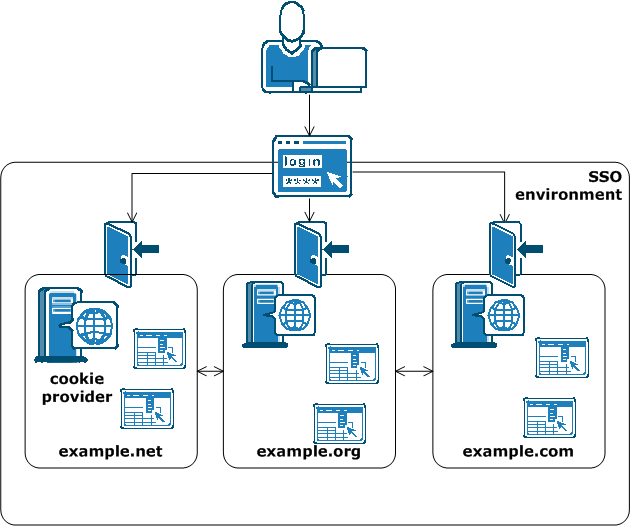
\includegraphics[scale=0.6]{sso-siteminder.png}
\caption{Exemplo de implementação de SSO do SiteMinder}
\label{fig:sso-siteminder}
\end{figure}

Este é apenas um exemplo de implementação, a solução SiteMinder é um sistema
centralizado de gerenciamento de acesso Web da empresa CA Tecnologies, que
implementa uma série de soluções e SSO.

\subsection{Quais soluções existem?}

Quais soluções estão disponíveis para quem quer implementar SSO? Segue
uma lista baseada no artigo da
Wikipedia~\footnote{http://en.wikipedia.org/wiki/List\_of\_single\_sign-on\_implementations}
com soluções em software livre para SSO:

\subsubsection{Accounts \& SSO}

Framework contendo um conjunto de componentes e bibliotecas para autenticação
de contas de usuários online em clientes Desktops, em sistemas Linux e POSIX.

Mais em:
\begin{itemize}
  \item{http://en.wikipedia.org/wiki/Accounts\_\&\_SSO}
\end{itemize}

\subsubsection{Central Authentication Service (CAS)}

Protocolo de Single Sign-on para a Web. O nome CAS refere-se também a uma
implementação deste mesmo protocolo. O fluxo que ocorre durante a autenticação
é o seguinte:

\begin{itemize}
\item{Cliente visita uma aplicação requisitando autenticação}
\item{A aplicação redireciona o Cliente para o CAS}
\item{CAS valida atenticidade do Cliente (geralmente contra um banco, Kerberos, Active Directory, etc)}
\item{Se a autenticação tem sucesso, CAS retorna o cliente para a aplicação, passando um ticket de segurança}
\item{A aplicação valida o ticket contactando CASC}
\item{AS then gives the application trusted information about whether a particular user has successfully authenticated}
\end{itemize}

A implementação oficial do CAS é em Java e mantido pelo grupo
JASIG~\footnote{http://www.jasig.org}, existem implementações oficiais do lado
cliente em várias linguagens, .NET, PHP, Perl, Apache, etc.

\begin{figure}[h]
\center
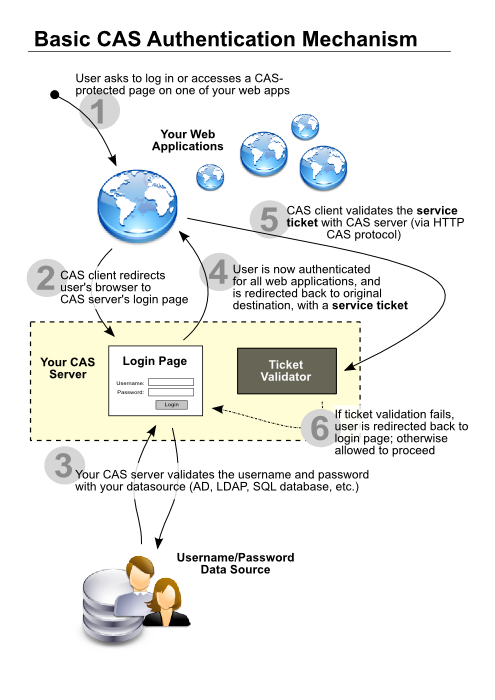
\includegraphics[scale=0.4]{sso-rubycas.png}
\caption{Diagrama do RubyCAS, implementação do protocolo CAS em Ruby}
\label{fig:sso-rubycas}
\end{figure}

%http://rubycas.github.io
%(tem pacote Debian)

Mais em:
\begin{itemize}
  \item{http://en.wikipedia.org/wiki/Central\_Authentication\_Service}
  \item{http://www.jasig.org/cas/protocol}
\end{itemize}

\subsubsection{Distributed Access Control System (DACS)}

DACS é um sistema de SSO leve combinado com mecanismos de autenticação e
controle de acesso para Web escrito em C/C++. Possui suporte para integrar com
diversos mecanismos de autenticação, como X.509, PAM, LDAP, etc. Possui módulo
de autenticação para servidor Web Apache.

%http://pdf.aminer.org/000/309/229/a_single_sign_on_protocol_for_distributed_web_applications_based.pdf

O Debian utiliza DACS para prover SSO entre alguns dos seus servidores para os
desenvolvedores do projeto, ver mais em:

Mais em:
\begin{itemize}
  \item{http://en.wikipedia.org/wiki/Distributed\_Access\_Control\_System\_(DACS)}
  \item{https://wiki.debian.org/DebianSingleSignOn}
\end{itemize}

\subsubsection{Enterprise Sign On Engine}

Plataforma de SSO, controle de acesso e federação compatível com SAML 2.0
e parcialmente compatível com
XACML~\footnote{http://en.wikipedia.org/wiki/XACML}.

Desenvolvido em Java e com suporte a Tomcat, Apache e IIS.

Mais em:
\begin{itemize}
  \item{http://en.wikipedia.org/wiki/Enterprise\_Sign\_On\_Engine}
\end{itemize}

\subsubsection{FreeIPA}

Solução da RedHat para SSO e "Policy and Audit". É comparável a solução
"Novell's Identity Manager" ou "Microsoft's Active Directory" pois tem
objetivos e mecanismos similares.

Usa as soluções: 389 Directory Server, MIT Kerberos 5, Apache HTTP e Python.

Na versão 3.0.0 usa Samba para integrar com Microsoft Active Directory.

Mais em:
\begin{itemize}
  \item{http://en.wikipedia.org/wiki/FreeIPA}
\end{itemize}

\subsubsection{IBM Enterprise Identity Mapping}

Framework para mapear identidades de usuários em várias plataformas distintas,
com poucas informações na Web, aparentemente apenas para integrar as soluçoes
da própria IBM.

Mais em:
\begin{itemize}
  \item{http://en.wikipedia.org/wiki/IBM\_Enterprise\_Identity\_Mapping}
\end{itemize}

\subsubsection{JBoss SSO}

Faz parte da suíte de soluções JBoss SOA, permite single sign-on e sign-off e
acesso federado a múltiplas aplicações e recursos computacionais em rede.

Dentre várias funcionalidades o JBoss SSO inclue:

\begin{itemize}
  \item{Interação entre aplicações e módulos baseados no padrão SAML}
  \item{Abordagem descentralizada}
  \item{Habilidade de conectar a diferentes sistemas de armazenamento}
\end{itemize}

Mais em:
\begin{itemize}
  \item{http://en.wikipedia.org/wiki/JBoss\_SSO}
\end{itemize}

\subsubsection{JOSSO}

Java Open Single Sign On (JOSSO) é uma solução de SSO para aplicações Web.
Baseado em Java EE. O framework permite mútiplos servidores web autenticar
usuários com suas credenciais. JOSSO se comunica com o armazenamento das
credenciais por LDAP ou JDBC. Fornece interface via SOAP sob o protocolo HTTP
para permitir fácil integração com aplicações não-Java.

Mais em:
\begin{itemize}
  \item{http://en.wikipedia.org/wiki/JOSSO}
\end{itemize}

\subsubsection{Kerberos}

Protocolo de autenticação em rede baseado em 'tickets para permitir nós se
comunicar sob uma rede não-segura para provar sua identidade para outro de
forma segura. Seus designers objetivaram principalmente como um modelo
cliente-servidor e isso provê autenticação tanto de usuários quanto de
servidores. Veja Figura~\ref{fig:kerberos} para exemplo de negociação com o
Kerberos.

\begin{figure}[h]
\center
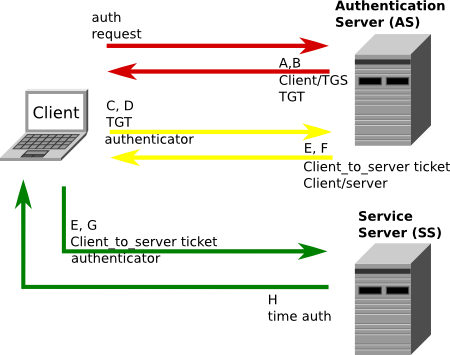
\includegraphics[scale=0.6]{kerberos.png}
\caption{Diagrama de negociação do Kerberos}
\label{fig:kerberos}
\end{figure}

Mais em:
\begin{itemize}
  \item{http://en.wikipedia.org/wiki/Kerberos\_(protocol)}
\end{itemize}

\subsubsection{OpenAM}

Provê single sign-on de forma transparente em infraestrutura de redes. Escrito
em Java, suporte a mais de 20 tipos de autenticação. Possui suporte a SAML e
emplementa sistema de autorização baseado em XACML. Veja exemplo na
Figura~\ref{fig:opensso} de uso do OpenAM em um portal de viagens.

\begin{figure}[h]
\center
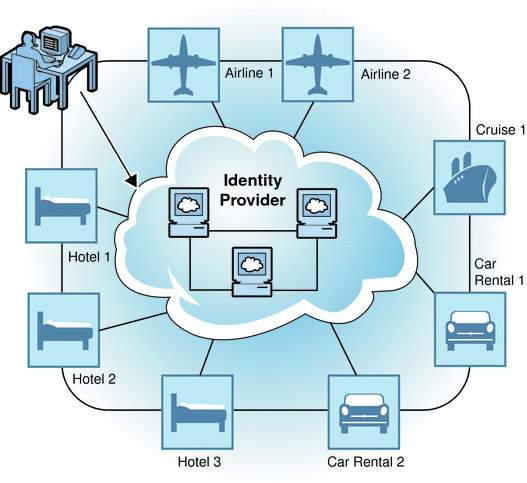
\includegraphics[scale=0.5]{opensso.png}
\caption{Exemplo de federação com OpenAM para um portal de viagens}
\label{fig:opensso}
\end{figure}

Mais em:
\begin{itemize}
  \item{http://en.wikipedia.org/wiki/OpenAM}
\end{itemize}

\subsubsection{Pubcookie}

Protocolo (e software) de SSO, o processo de autenticação se dá da seguinte
forma:

\begin{itemize}
  \item{Quando usuário acessa a aplicação, Pubcookie seta 2 cookies, pré-sessão e concessão de requisição}
  \item{Redireciona usuário para página de login}
  \item{Usuário fornece login e senha, se o login for com sucesso, seta 2 cookies, login e concessão}
\end{itemize}

O ultimo release do projeto é de 2010, um pouco antigo.

Mais em:
\begin{itemize}
  \item{http://en.wikipedia.org/wiki/Pubcookie}
\end{itemize}

\subsubsection{SAML}

Linguagem de marcação para definir comunicação sobre autenticação e autorização

Security Assertion Markup Language (SAML) é uma linguagem de marcação baseada
em XML para troca de dados de autenticação e autorização definido pelo OASIS
Security Services Technical Committee. O SAML é principalmente desenvolvido
para ser aplicado em web browser single sign-on.

A especificação SAML define 3 papéis:
\begin{itemize}
  \item{o principal (tipicamente um usuário)}
  \item{o provedor de identidade (IdP)}
  \item{o provedor de serviço (SP)}
\end{itemize}

A interação entre eles está representada na Figura~\ref{fig:saml2}.

\begin{figure}[h]
\center
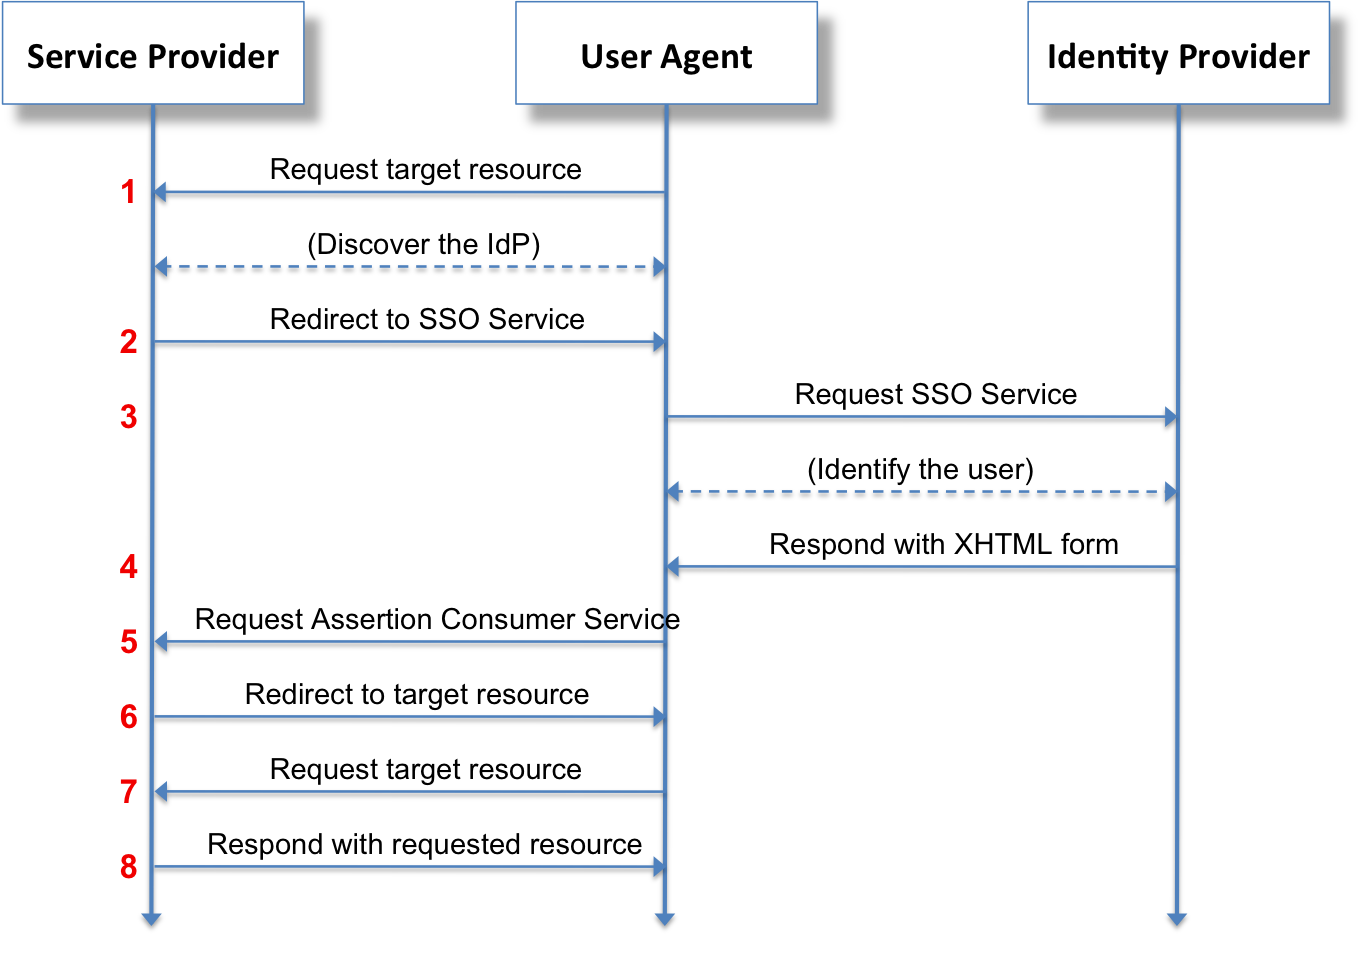
\includegraphics[scale=0.5]{saml2.png}
\caption{Single Sign-on com SAML2}
\label{fig:saml2}
\end{figure}

Mais em:
\begin{itemize}
  \item{http://en.wikipedia.org/wiki/Security\_Assertion\_Markup\_Language}
\end{itemize}

\subsubsection{Shibboleth}

Middleware para SSO e autenticação baseado em SAML.

Mais em:
\begin{itemize}
  \item{http://en.wikipedia.org/wiki/Shibboleth\_(Internet2)}
\end{itemize}

\subsubsection{ZXID}

kit de gerenciamento de identidade SAML 2.0

Compatícel co SAML 2.0, Liberty ID-WSF 2.0 e XACML 2.0. Implementado em C com
poucas dependencias externas, com bibliotecas para PHP, Perl e Java via SWIG.

Mais em:
\begin{itemize}
  \item{http://en.wikipedia.org/wiki/ZXID}
\end{itemize}

\section{IdP - Identity Provider}

\subsection{O que é IdP?}

Identity Provider, ou Provedor de Identidade, é um serviço responsável por
gerenciar informações de identidade entre sistemas, usuários ou outros atores,
provendo através de um módulo interno ou externo serviço de autenticação e
autorização de forma segura afim de verificar a autenticidade dos atores,
normalmente usuários.

Um provedor de identidade fornece uma alternativa para que vários serviços web
distintos autentiquem seus usuários através dele, de forma que um usuário pode
ter apenas um login/senha e autentique em vários serviços com este mesmo
login/senha. Isto não implica em Single Sign-on, pois com um provedor de
identidade apenas o usuário ainda precisa passar por uma etapa de
autenticação, num ambiente de SSO isto fica transparente e o usuário ao logar
num sistema Web não precisa passar pela etapa de autenticação ao acessar um
segundo serviço.

Uma solução de SSO é composta usualmente de ao menos 3 componentes:

\begin{itemize}
  \item{Usuário/cliente, geralmente usa-se os termo {\it Principal}}
  \item{Provedor de identidade, {\it IdP - Identity Provider}}
  \item{Provedor de serviço}
\end{itemize}

Em um ambiente SSO um usuário autentica apenas uma vez e um token de segurança
é passado entre os sistemas participantes do ambiente de SSO. Normalmente
suportam os tipos de token de segurança mais comuns, como:

\begin{itemize}
  \item{SAML}
  \item{SPNEGO}
  \item{X.509}
\end{itemize}

Um provedor de identidade (IdP) sozinho não garante Single Sign-on (SSO), um
IdP é normalmente parte de um ambiente de SSO, normalmente um primeiro passo
para ter um ambiente SSO é implantar um serviço de IdP.

Definição de IdP segundo a OASIS:

\begin{itemize}
  \item{http://en.wikipedia.org/wiki/Identity\_provider}
\end{itemize}

Mais sobre esses termos pode ser encontrado em:
\begin{itemize}
  \item{http://www.empowerid.com/learningcenter/technologies/service-identity-providers}
\end{itemize}

Mais sobre Identity Provider em:
\begin{itemize}
  \item{http://en.wikipedia.org/wiki/Identity\_provider}
\end{itemize}

\subsection{IdP no Noosfero}

O Noosfero não implementa oficialmente integração de nenhum protocolo ou
tecnologia de provedor de identidade, no entando existe uma implementação
não-oficial em uso na rede Cirandas.net~\footnote{http://cirandas.net} de uso
do OAuth e do Mozilla Persona, o código fonte desta implementação não-oficial,
ainda não integrada ao repositório oficial do Noosfero na seguinte URL:

\begin{itemize}
  \item{https://github.com/CIRANDAS/noosfero-ecosol/tree/master/plugins/oauth}
\end{itemize}

\subsection{Resolve qual problema?}

Um usuário criar apenas um registro login/senha e acessa múltiplos serviços
através deste mesmo login/senha, sem necessidade de ter várias senhas em cada
serviço Web que deseje acessar, isso facilita por exemplo quando o usuário
precisa alterar sua senha, pois em apenas um único ponto ele altera a senha de
acesso a diversos sistemas, de uma só vez.

%\subsection{Como funciona?}

\subsection{Quais soluções existem?}

\subsubsection{Mozilla Persona}

O Mozilla Persona é um sistema de autenticação descentralizado, projeto
iniciado em 2011 e compartilha alguns dos objetivos de sistemas similares como
OpenID ou Facebook Connect, mas com algumas diferenças:

\begin{itemize}
  \item{Usa endereços de email como identificador}
  \item{Foco na privacidade do usuário}
  \item{Forte integração com navegadores web}
\end{itemize}

A motivação pela privacidade está no fato de que um provedor de identidade não
deve saber quais sites o usuário está se identificando.

Mais em:
\begin{itemize}
  \item{http://en.wikipedia.org/wiki/Mozilla\_Persona}
\end{itemize}

Thread sobre SSO com Persona:
   * https://groups.google.com/forum/\#!topic/mozilla.dev.identity/oNseXZxbVUQ

Baseado no protocolo BrowserID prototipado pela Mozilla.
* http://identity.mozilla.com/post/7616727542/introducing-browserid-a-better-way-to-sign-in

A Mozilla disponibiliza uma instancia do Persona rodando em:

\begin{itemize}
  \item{https://login.persona.org}
\end{itemize}

Mas é possível rodar um proprio servidor Persona seguindo a seguinte
instruções:

\begin{itemize}
  \item{https://developer.mozilla.org/en-US/Persona/Implementing\_a\_Persona\_IdP}
\end{itemize}

\subsubsection{OAuth}

OAuth é um padrão aberto para autorização, desenhado especialmente para
funcionar sob o protocolo HTTP, OAuth essencialmente permite acesso a tokens
gerados por servidores de autorização. O cliente usa o token de acesso para
acessar serviços protegidos. Ele é complementar, apesar de distinto, do OpenID.

A maioria dos grandes serviços para Web implementam ele, como: Google,
Facebook, Yahoo, AOL, Microsoft, PayPal, MySpace, and Flickr entre outros.
Ainda, a maioria dos serviços de email provêem serviço de autorização via
OAuth.

Mais em:
\begin{itemize}
  \item{http://en.wikipedia.org/wiki/OAuth}
\end{itemize}

Existem algumas preocupações com o OAuth como descrito no link abaixo, alguns
dos autores iniciais do protocolo saíram do projeto apontando uma série de
falhas no protocolo, mas não chegam a recomendar o desuso dele, apenas apontam
para um novo e melhor caminho que não é possível incluir no OAuth por força
das organizações que fazem partem do comitê que define o padrão, um deles é o
Eran Hammer que propôs duas novas soluções, Oz e o Hawk.

\begin{itemize}
  \item{http://hueniverse.com/2012/07/26/oauth-2-0-and-the-road-to-hell}
  \item{https://github.com/hueniverse/oz}
  \item{https://github.com/hueniverse/hawk}
\end{itemize}

\subsubsection{OpenID}

Sistema de identificação baseado em URL. Permite autenticação de usuários
usando parceiros para autenticação, usuários podem criar seu acesso onde
desejar e logar onde quer que OpenID seja suportado.

Usuários podem criar contas com seu provedor de identidade OpenID preferido e
então usar sua conta para logar em qualquer outro sistema Web que aceite
autenticação com OpenID. Alguns provedores de OpenID hoje são: Google, Yahoo!,
PayPal, BBC, AOL, LiveJournal, MySpace, IBM, etc.

O sistema que influenciou identificação baseado em URL no OpenID foi o LID:

\begin{itemize}
  \item{http://en.wikipedia.org/wiki/Light-Weight\_Identity}
\end{itemize}

Mais em:
\begin{itemize}
  \item{http://en.wikipedia.org/wiki/OpenID}
\end{itemize}

\subsubsection{OpenID Connect}

Camada de autenticação em cima do OAuth 2.0, um framework de autorização,
promovido pelo OpenID Foundation.

Mais em:
\begin{itemize}
  \item{http://en.wikipedia.org/wiki/OpenID\_Connect}
\end{itemize}

%% \subsubsection{WS-Federation}
%% 
%% Parte da especificação de identificação federada da iniciativa WS-Security:
%% 
%% \begin{itemize}
%%   \item{http://en.wikipedia.org/wiki/WS-Federation}
%% \end{itemize}
%% 
%% WS-Security, WS-Trust e WS-SecurityPolicy provêem um modelo básico de
%% federação entre provedores de identidade. Estas especificações definem
%% mecanismos para 
%% 
%% WS-Security, WS-Trust, and WS-SecurityPolicy provide a basic model for federation between Identity
%% Providers and Relying Parties. These specifications define mechanisms for codifying claims (assertions)
%% about a requestor as security tokens which can be used to protect and authorize web services requests
%% in accordance with policy. WS-Federation extends this foundation by describing how the claim
%% transformation model inherent in security token exchanges can enable richer trust relationships and
%% advanced federation of services. This enables high value scenarios where authorized access to resources
%% managed in one realm can be provided to security principals whose identities and attributes are
%% managed in other realms. WS-Federation includes mechanisms for brokering of identity, attribute
%% discovery and retrieval, authentication and authorization claims between federation partners, and
%% protecting the privacy of these claims across organizational boundaries. These mechanisms are defined
%% as extensions to the Security Token Service (STS) model defined in WS-Trust. In addition WS-Federation
%% defines a mapping of these mechanisms, and the WS-Trust token issuance messages, onto HTTP such
%% that WS-Federation can be leveraged within Web browser environments. The intention is to provide a
%% common infrastructure for performing Federated Identity operations for both web services and
%% browser-based applications. A common protocol provides economies with regard to development,
%% testing, deployment and maintenance for vendors and customers alike.
%% 
%% Fonte: http://download.boulder.ibm.com/ibmdl/pub/software/dw/specs/ws-fed/WS-FederationSpec05282007.pdf?S\_TACT=105AGX04\&S\_CMP=LP

\section{Outras iniciativas}

\subsection{OpenAthens - Reino Unido}

Athens, iniciativa do Reino Unido, iniciou em instituições de ensino
universidades e então pelas instituições de saúde, adota SAML e interfaces via
Shibboleth. Em funcionamento desde 1996 com mais de 4.5 milhões de contas de
usuários é usado para prover acesso a mais de 300 serviços web distintos,
entre universidades e serviços públicos.

Desenvolvido pela empresa Eduserv, uma empresa sem fins lucrativos sediada em
Bath-UK:

\begin{itemize}
  \item{http://www.eduserv.org.uk/services/OpenAthens}
\end{itemize}

O post no link abaixo fornece uma visão clara de como tudo funciona:

\begin{itemize}
  \item{http://everything2.com/index.pl?node\_id=1888399}
\end{itemize}

Mais em:
\begin{itemize}
  \item{http://en.wikipedia.org/wiki/Athens\_access\_and\_identity\_management}
\end{itemize}

\subsection{Microsoft account}

O Microsoft account, anteriormente conhecido como Windows Live ID é um
provedor de identidade para os serviços da Microsoft, está sendo cidado aqui
apenas para exemplificar uma solução não-livre em produção, existem outras,
como o próprio Facebook Connect. O Microsoft account implementa OpenID e é
também um provedor de identidade OpenID.

Mais em:
\begin{itemize}
  \item{http://en.wikipedia.org/wiki/Microsoft\_account}
\end{itemize}

\subsection{Liberty Alliance}

Iniciativa entre organizações para promover padrões de federação, IGF,
serviços de identidade, etc... submeteu para o OASIS Group a especificação do
SAML 2.0, propôs uma séries de soluções como: OpenAz, ZXID, etc... As
iniciativas deste grupo hoje estão sendo mantidas pelo Kantara Initiative.

Mais em:
\begin{itemize}
  \item{http://en.wikipedia.org/wiki/Liberty\_Alliance}
  \item{https://en.wikipedia.org/wiki/Kantara\_Initiative}
\end{itemize}

\section{Discussão}

Discussao sobre CAS x OAuth:
* http://stackoverflow.com/questions/2033026/sso-with-cas-or-oauth/3181557\#3181557

CAS centraliza a autenticação, deve ser usado quando todas as aplicações
autenticam numa mesma base de credenciais usuário/senha de usuários.

OpenID decentraliza a autenticação, deve ser usado para aceitar login de
qualquer provedor OpenID, mas a aplicação pode restringir quais provedores
OpenID aceitar no entando.

Nem CAS nem OpenID lidam com autorização nativamente.

OAuth lida com autorização, autoriza por exemplo que um site X possa efetuar
autenticação a partir de um serviço de autenticação de terceiros Y. OAuth é
sobre permitir usuário controlar como seus recursos serão acessados por
terceiros.

CAS a partir da versão 3.5 suporta OAuth cliente e
servidor~\footnote{https://wiki.jasig.org/display/CASUM/OAuth}.

CASE: OpenSSO foi utilizado pela CPqD para implantas SSO entre diversar aplicações
da empresa https://blogs.oracle.com/superpat/entry/opensso\_at\_cpqd

CAS é geralmente a escolhe preferida para grande organizações, onde se quer
centralizar a base de usuários, exemplo universidades.

Falha grave de segurança:
* http://research.microsoft.com/apps/pubs/default.aspx?id=160659

Discussao na visao do pessoal do DACS sobre o porque SSO é pouco adotado no
geral:
* http://dacs.dss.ca/about.html

\subsection{Iniciativas (Governo e Comunidade)}

\subsubsection{Login Cidadão}

Projeto piloto desenvolvido pela PROCERGS de um provedor de identidade com
base em OAuth para os serviços do governo do estado do Rio Grande do Sul.

Instancia do Login Cidadão rodandm em:
\begin{itemize}
  \item{https://meu.rs.gov.br}
\end{itemize}

Código fonte, projeto desenvolvido em PHP com framework symfony:
\begin{itemize}
  \item{https://github.com/PROCERGS/login-cidadao}
\end{itemize}

A equipe responsável pelo Login Cidadão esteve no Fisl15 apresentando a
palestra "Login Cidadão: Uma conta. Tudo o que o governo oferece", o vídeo
está disponível através do link abaixo:
\begin{itemize}
  \item{http://hemingway.softwarelivre.org/fisl15/high/41f/sala41f-high-201405081612.ogv}
\end{itemize}

\subsubsection{Id da Cultura}

O MinC (Ministério da Cultura) iniciou um projeto de provedor OpenID para
fornecer identidade centralizada para os serviços Web do MinC e parceiros, o
projeto é desenvolvido em Python e o código-fonte está disponível em:
\begin{itemize}
  \item{https://github.com/hacklabr/iddacultura-provider}
\end{itemize}

Esta implementação foi posteriormente aproveitada pelo projeto Mapas Culturais
do Estado de São Paulo e hoje está sendo utilizado neste projeto, o código
utilizado neste projeto está em:
\begin{itemize}
  \item{https://github.com/hacklabr/mapasculturais-openid}
\end{itemize}

\subsection{Proposta para o Participa.BR}

Qual caminho tomar?

Neste contexto de SSO, o Participa.BR tem a necessidade de criar um
arranjo de confiança entre alguns sites relacionados ao projeto, inicialmente
estes os sites que farão parte deste arranjo são, além do próprio Participa.br
são:

\begin{itemize}
  \item{Participatório (gov)}
  \item{Cidade Democrática (org)}
  \item{Cultura Educa (cc/org)}
\end{itemize}

Assim que implementado conectaríamos:

O caminho de implementação pode ser SLTI (gov) ou Serpro (gov/com).

\section{Considerações finais}

Neste documento foi apresentado um \ProductDescription

Lembramos que para tornar o Portal de Consulta Pública realmente um canal de
consulta e participação popular na discussão e na definição da agenda
prioritária do país, é necessário que além de documentação faça-se um esforço
de movimentar as pessoar fora do ambiente virtual, para que haja um
engajamento no uso e contribuição deste projeto de forma consistente e perene.

\vspace{1cm}

Sem mais nada a acrescentar, coloco-me à disposição.

\vspace{1cm}

\begin{minipage}{\textwidth}
  Brasília/DF, \DiaEntrega \ de \MesEntrega\\[1cm]
  \textbf{\MyName}\\
  \small Consultor do PNUD
\end{minipage}

\end{document}
